\section{ロボット競技大会の概要}\label{ux30edux30dcux30c3ux30c8ux7af6ux6280ux5927ux4f1aux306eux6982ux8981}

筆者は8月に川崎市で開催されるかわさきロボット競技大会というロボットコンテストに参加しています。
四角いリング上で2台のロボットに戦わせる対戦式の大会です。
(Fig.\ref{fig34})
ラジコンでよく使われるプロポでロボットを操作し、相手の機体をリング場外へ押し出すか、ダウンさせた後10カウント状態をキープすれば勝利となります。

\begin{figure}[htbp]
\centering
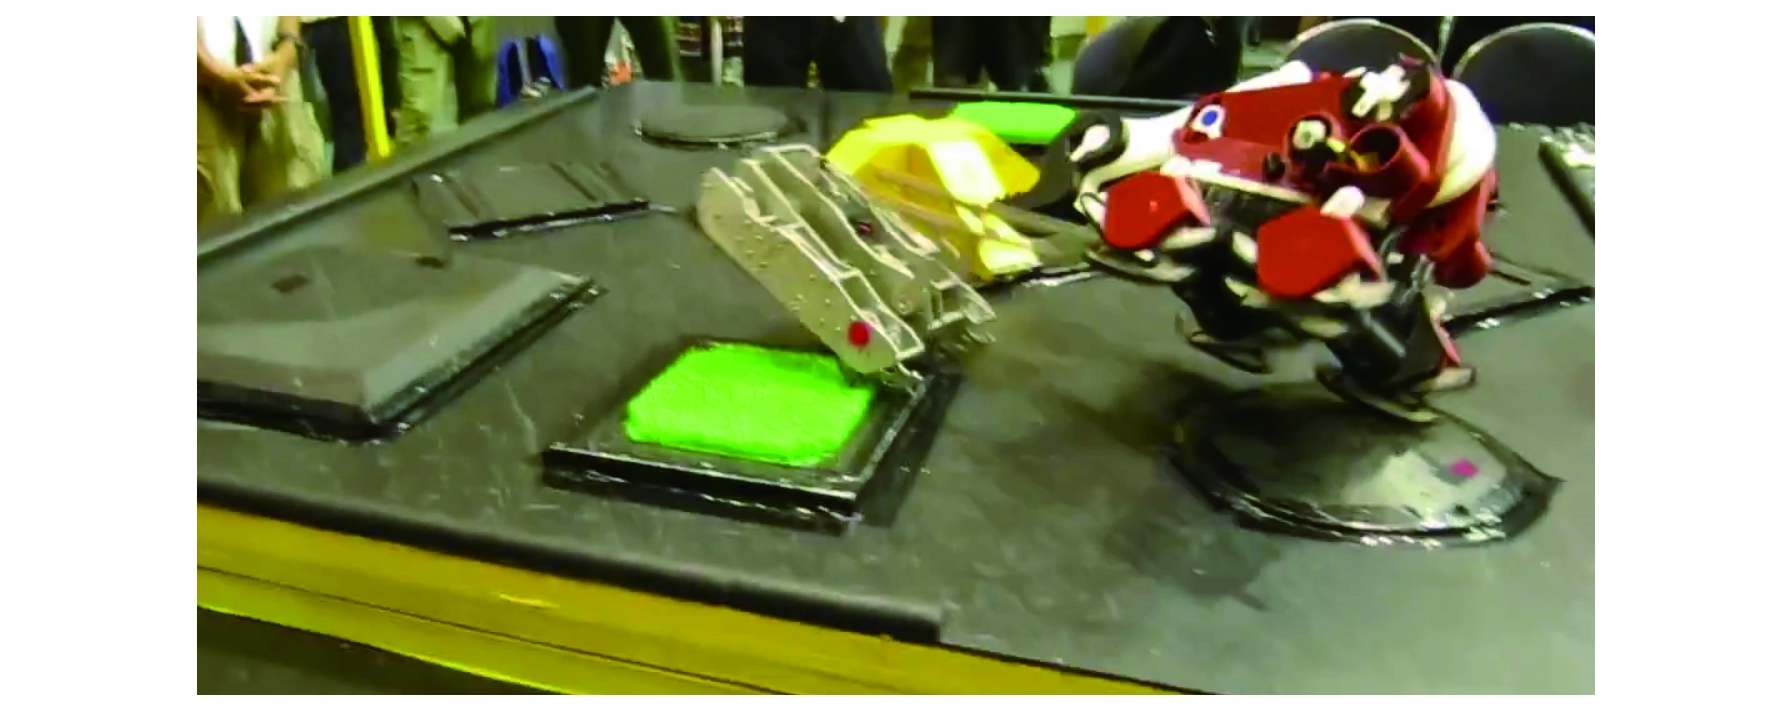
\includegraphics[width=380pt]{fig/fig34_cmyk.jpg}
\caption{かわさきロボット大会の様子}
\label{fig34}
\end{figure}

機体仕様には規定があります。以下に本体構成に関わる項目を列挙します。
以下のルールは2014年時に参加した時のものです。
現在は規則に幾つか変更が入っているため、詳細はかわさきロボット競技大会公式サイト\cite{kawasaki_public_HP}ご参照ください。

\begin{itemize}
\tightlist
\item
  サイズ制限:幅250mm×奥行350mm×高さ700mm(待機時)
\item
  重量制限:3500g以内
\item
  ロボットには、それぞれ1セット以上の脚機構、アーム機構が搭載されていること
\item
  脚部は、往復運動を行う部位を接地部として、リンク機構を用いて移動するように設計されていること
\item
  アーム部は、機構のみを用いて物体をアームで移動させることができ、大会が規定する揺動リンク機構を有し、高さ200mm地点を通過すること
\end{itemize}

\section{構想設計}\label{ux69cbux60f3ux8a2dux8a08}

\subsection{コンセプト}\label{ux30b3ux30f3ux30bbux30d7ux30c8}

2014年度のかわさきロボット競技大会では、筆者は下記のようにコンセプトを決めました。

\begin{enumerate}
\def\labelenumi{\arabic{enumi}.}
\tightlist
\item
  大会上、今までに無い機体を作りたい(新規性)
\item
  3Dプリンタでほぼ全ての部品を作る(見た目の分かりやすさ)
\item
  強度担保のため、極力シンプルな機構で構成する(実現性)
\end{enumerate}

今思い返すと3Dプリンタを活用することそのものが目的になっていました。
趣味だからこそできることですね。

\subsection{全体構成}\label{ux5168ux4f53ux69cbux6210}

上記コンセプトをもとにポンチ絵を描きました。(Fig.\ref{fig01})
細かい部分は考えず、全体の大きな構成を見通したいので、ざっくりした絵になっています。

個人的にはポンチ絵を描くツールはなんでもよいと考えています。
今回は、Excelのオートシェイプ機能を使って書きました。
手書きでもよいかと思います。

ポンチ絵を描きながら下記項目をまとめていきました。

\begin{itemize}
\tightlist
\item
  フレーム構造:底部フレームに側面フレームを取り付け、コの字型にすることで強度アップする。
\item
  脚部:4か所の脚部は全て共通化し、メンテナンス性を向上させる。取り付けは底部フレームとする。
\item
  アーム:相手機体と直接接触が多い個所なので、メンテナンス性(交換のしやすさ)が求められる。簡単に組み立て、分解ができるよう、側面フレームだけに取り付ける。
\item
  電装系:電装系は底部フレーム上に取り付ける。また、相手機体のアームが電装系に当たってしまうと動かなくなってしまうリスクがあるため、一旦組み立ててしまえば外からはアクセスできなようにする。
   \\

  \begin{figure}[htbp]
  \centering
  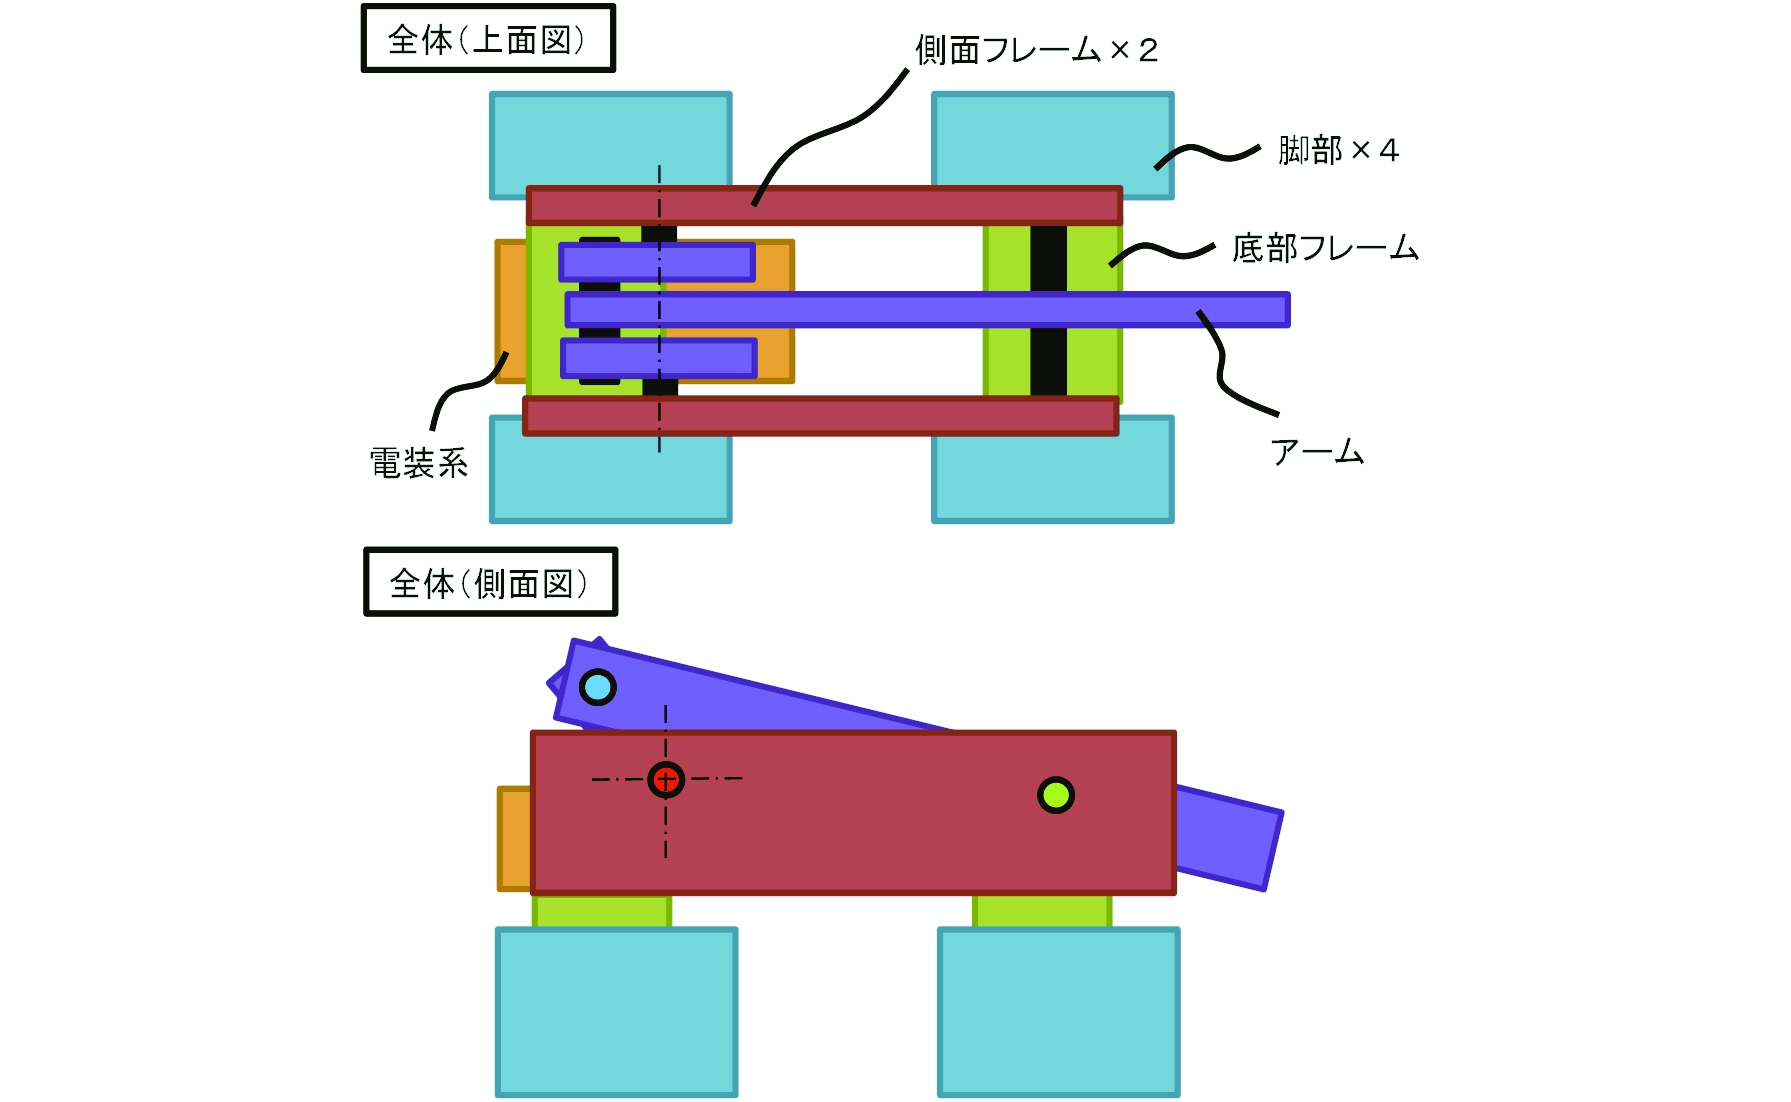
\includegraphics[width=380pt]{fig/fig01_cmyk.jpg}
  \caption{全体構成 ポンチ絵}
  \label{fig01}
  \end{figure}
\end{itemize}

\subsection{脚構成}\label{ux811aux69cbux6210}

\begin{itemize}
\tightlist
\item
  リンク機構:シンプルなスライダリンク機構を採用し、低強度な部品でも問題が出ないようにする
\item
  脚厚み:足先は走行時の衝撃が加わるため、なるべく厚くして強度アップを狙う
\item
  脚個数:一つの脚部には足を3枚用いる。足は位相を120°ずつずらして並列に配置することで、常に足先を地面に接地させる。これによりロボットの上下振動が抑えられ、走破性が良化する
\end{itemize}

\begin{figure}[htbp]
\centering
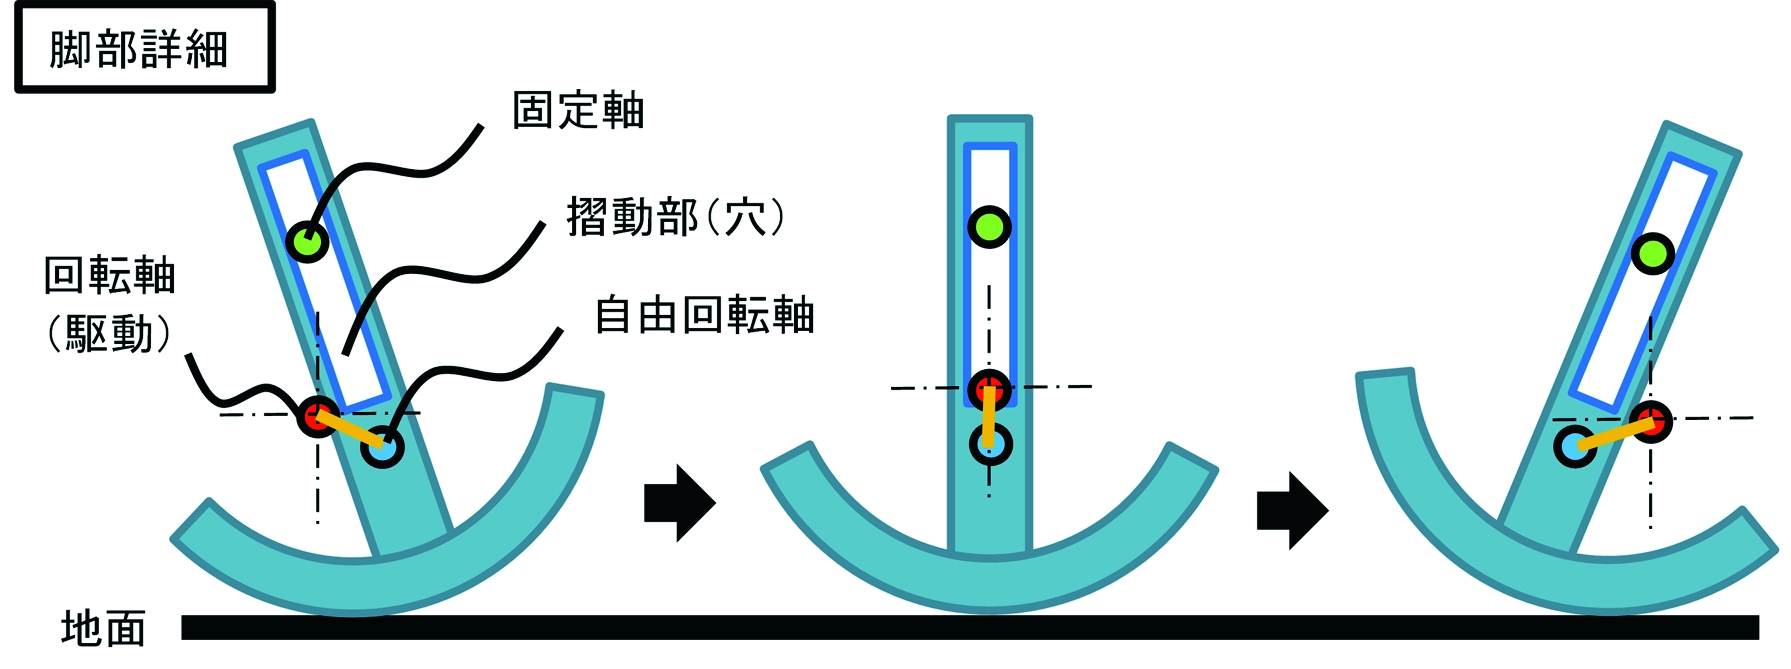
\includegraphics[width=300pt]{fig/fig02_cmyk.jpg}
\caption{脚構成 ポンチ絵}
\label{fig02}
\end{figure}

\subsection{アーム構成}\label{ux30a2ux30fcux30e0ux69cbux6210}

\begin{itemize}
\tightlist
\item
  リンク機構:スライダリンク機構を利用する。シンプルな構成であるため、強度の弱い材料で作っても問題が出にくいと考えた。
\item
  厚み:アームは相手機体と当接する部分なので、なるべく厚くし強度アップを狙う。
\item
  見た目:アームは機体の中でも最も目立つ部分。詳細設計時にはデザインにこだわる。
\end{itemize}

\begin{figure}[htbp]
\centering
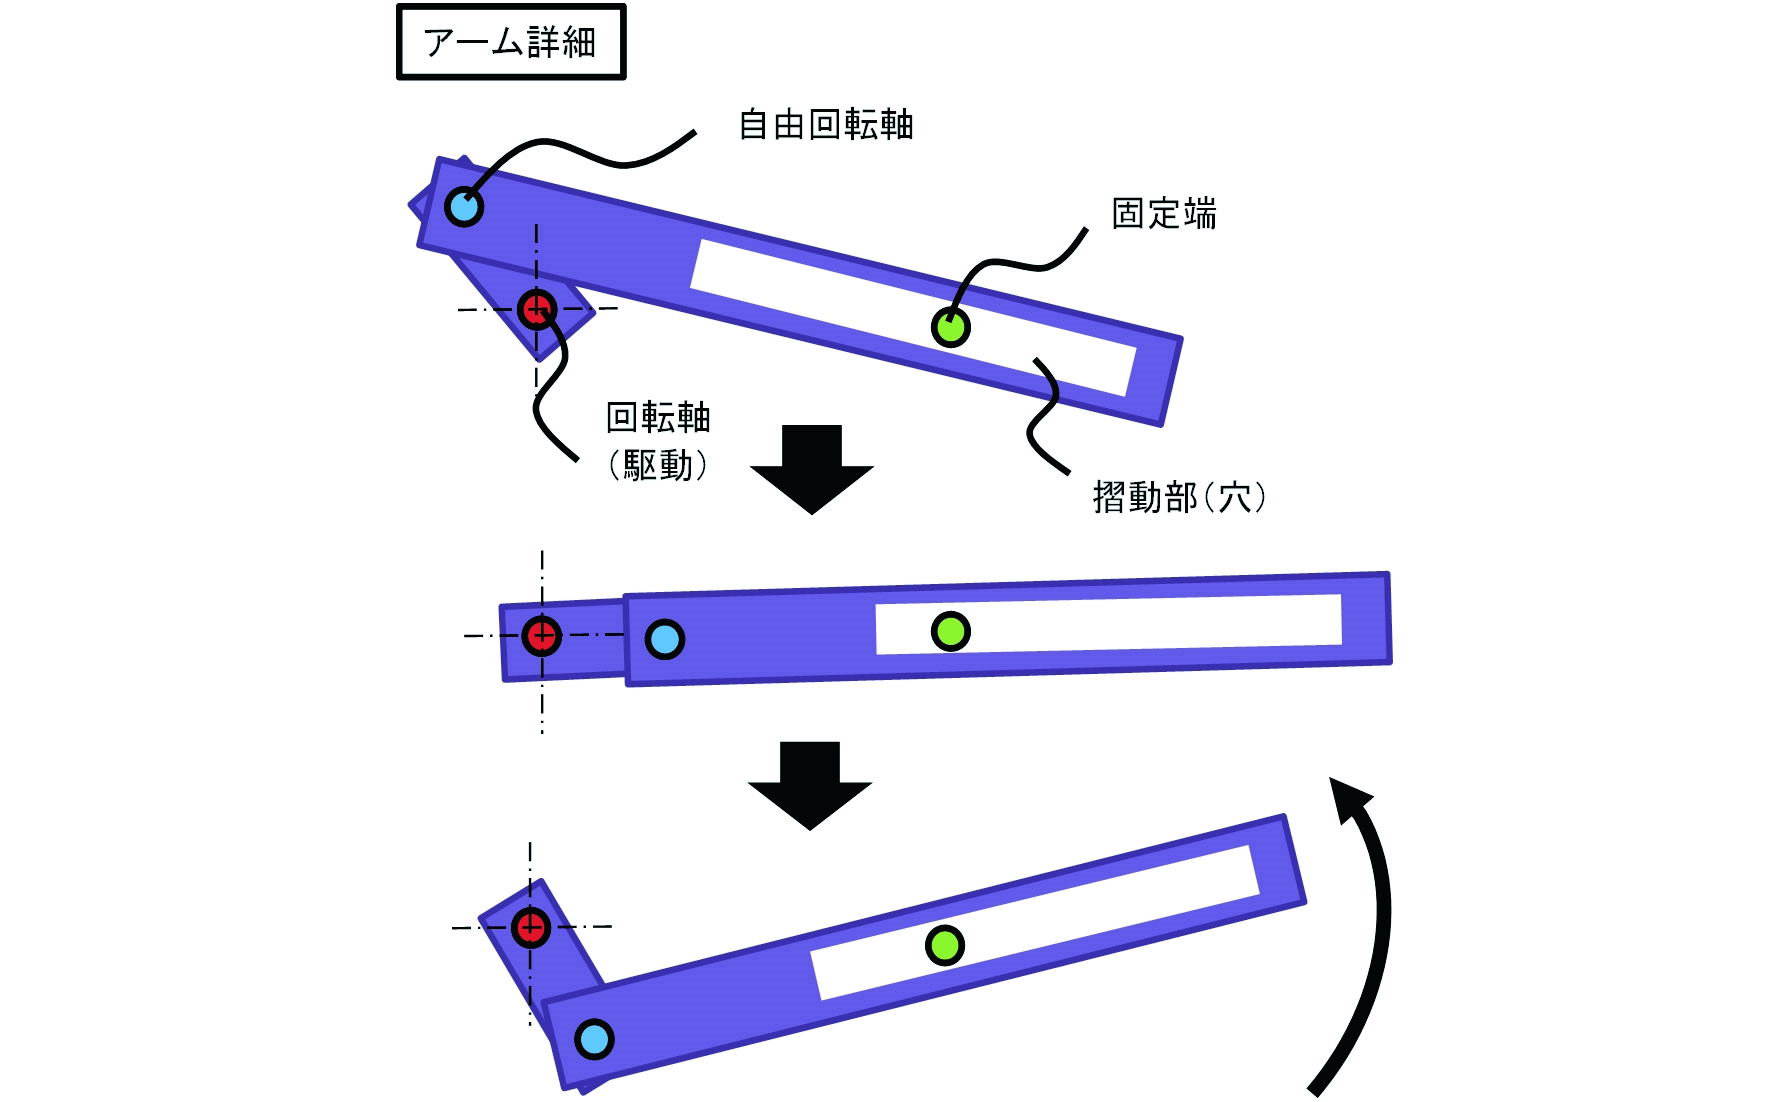
\includegraphics[width=380pt]{fig/fig03_cmyk.jpg}
\caption{アーム構成 ポンチ絵}
\label{fig03}
\end{figure}

\subsection{レイアウト設計}\label{ux30ecux30a4ux30a2ux30a6ux30c8ux8a2dux8a08}

構想設計が終わった後、レイアウト設計に移ります。
構成設計ではサイズ感が分からないため、規定サイズを念頭に置きながら大まかな機体サイズを決めていきます。
流れは下記の通りです。

\begin{itemize}
\tightlist
\item
  大会の規格サイズを確認:規定(2014年度)では機体サイズは幅250mm×奥行350mm×高さ700mm以内(停止時)
\item
  ポンチ絵をブロックで作成:感覚でユニットのサイズを決めてブロックを作成。細かい部品は作成しません。
\item
  ブロックを配置:規格サイズに合わせて、ユニットブロックをレイアウト
\end{itemize}

私が行った実例をFig.\ref{fig04}に示します。
ここまでいくと、脚部で使用できるスペースや、アームのサイズ感など、大まかに把握することができます。

使用したツールはCreo
Elements\cite{creo_elements}です。個人利用の範囲内なら無料で使用できます。

\begin{figure}[htbp]
\centering
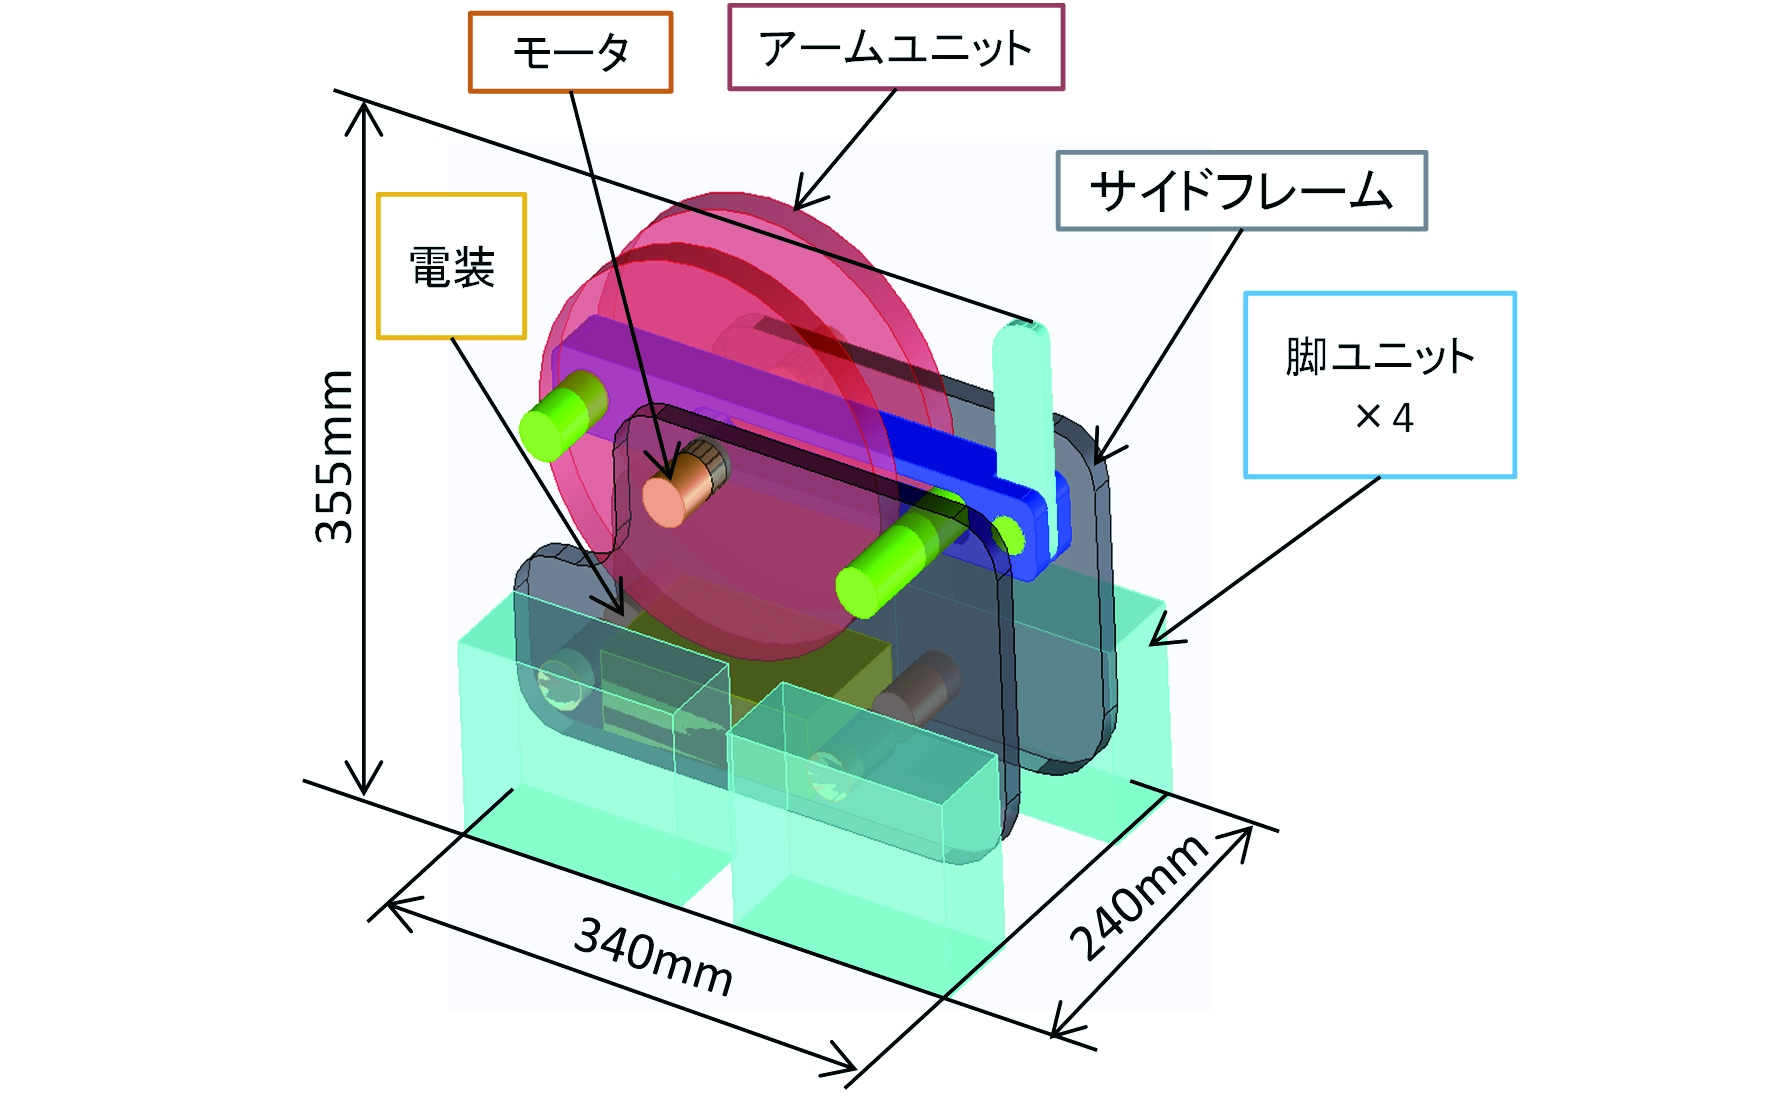
\includegraphics[width=380pt]{fig/fig04_cmyk.jpg}
\caption{レイアウト設計}
\label{fig04}
\end{figure}

\section{基本設計}\label{ux57faux672cux8a2dux8a08}

基本設計では構想設計を具体化するため、まずアクションアイテムを書き出しました。
3Dプリンタをフル活用するつもりでしたので、最も力が加わるアーム設計をケアした内容になっています。

\begin{enumerate}
\def\labelenumi{\arabic{enumi}.}
\tightlist
\item
  アーム設計パラメータ:大会規定と目標値から、各種設計パラメータを設定する
\item
  アーム強度計算:3Dプリンタによる部品で相手機体を持ち上げた時、破損しないように強度計算を行い、部品厚みを決定する
\item
  積層方向の割れ防止構成:3Dプリンタ積層方向に高負荷がかかると割れが発生しやすい。積層方向に力がかかる部品に関しては強度アップ構成を考える。
\item
  モータ出力部の削れ防止構成:モータ出力部と締結する3Dプリンタ部品が削れ、駆動伝達できなくなるリスクがある。信頼性の高い締結構成を考える。
\item
  大型部品の分割構成:3Dプリンタで作成できる部品サイズは、プリンタのテーブルサイズで決まる。大型部品の分割方法と締結方法を考える。
\end{enumerate}

\subsection{アーム設計パラメータ}\label{ux30a2ux30fcux30e0ux8a2dux8a08ux30d1ux30e9ux30e1ux30fcux30bf}

アーム設計パラメータとして、リンク機構の位置、クランク長さ、モータ個数、減速比があります。
対戦相手との間合いや持ち上げ高さ、等から決めるので、まずは目標値を定めました。

\begin{itemize}
\tightlist
\item
  アームの射程距離:作用点位置を機体前面から250mmとする
\item
  相手機体持ち上げ高さ:大会規格の200mm地点を通過する
\item
  相手機体持ち上げ力:3500g(機体重量の大会規格)を持ち上げる
\end{itemize}

\subsubsection{アーム設計パラメータ 計算モデル}\label{ux30a2ux30fcux30e0ux8a2dux8a08ux30d1ux30e9ux30e1ux30fcux30bfux8a08ux7b97ux30e2ux30c7ux30eb}

設計パラメータは相互に影響しあうため、独立して一つ一つを決定していくことが困難です。
例えば、アームの射程距離を短くすれば必要なモータ駆動力は少なくてよいが、アーム作用点の通過高さは低くなります。
一方で、アームの射程距離を長くすると必要なモータ駆動力も多く必要となり、アーム作用点の通過高さは高くなります。
そこで、各種パラメータを可視化&持ち上げ力計算ツールをExcelで作りました(Fig.\ref{fig05})。

\begin{itemize}
\tightlist
\item
  アームに駆動を与えるポイントを原点Oに設定
\item
  第1クランク部品の長さをL1とし、第2クランク部品の長さをL2と設定
\item
  第1クランク部品と第2クランク部品の接続ポイントを中間自由回転軸aに設定
\item
  第2クランク部品に設けた長穴と摺動するポイントを中間固定軸jに設定
\item
  作用点をcと設定し、作用力を計算から算出
\item
  駆動力の伝達力損失は無視
\end{itemize}

\begin{figure}[htbp]
\centering
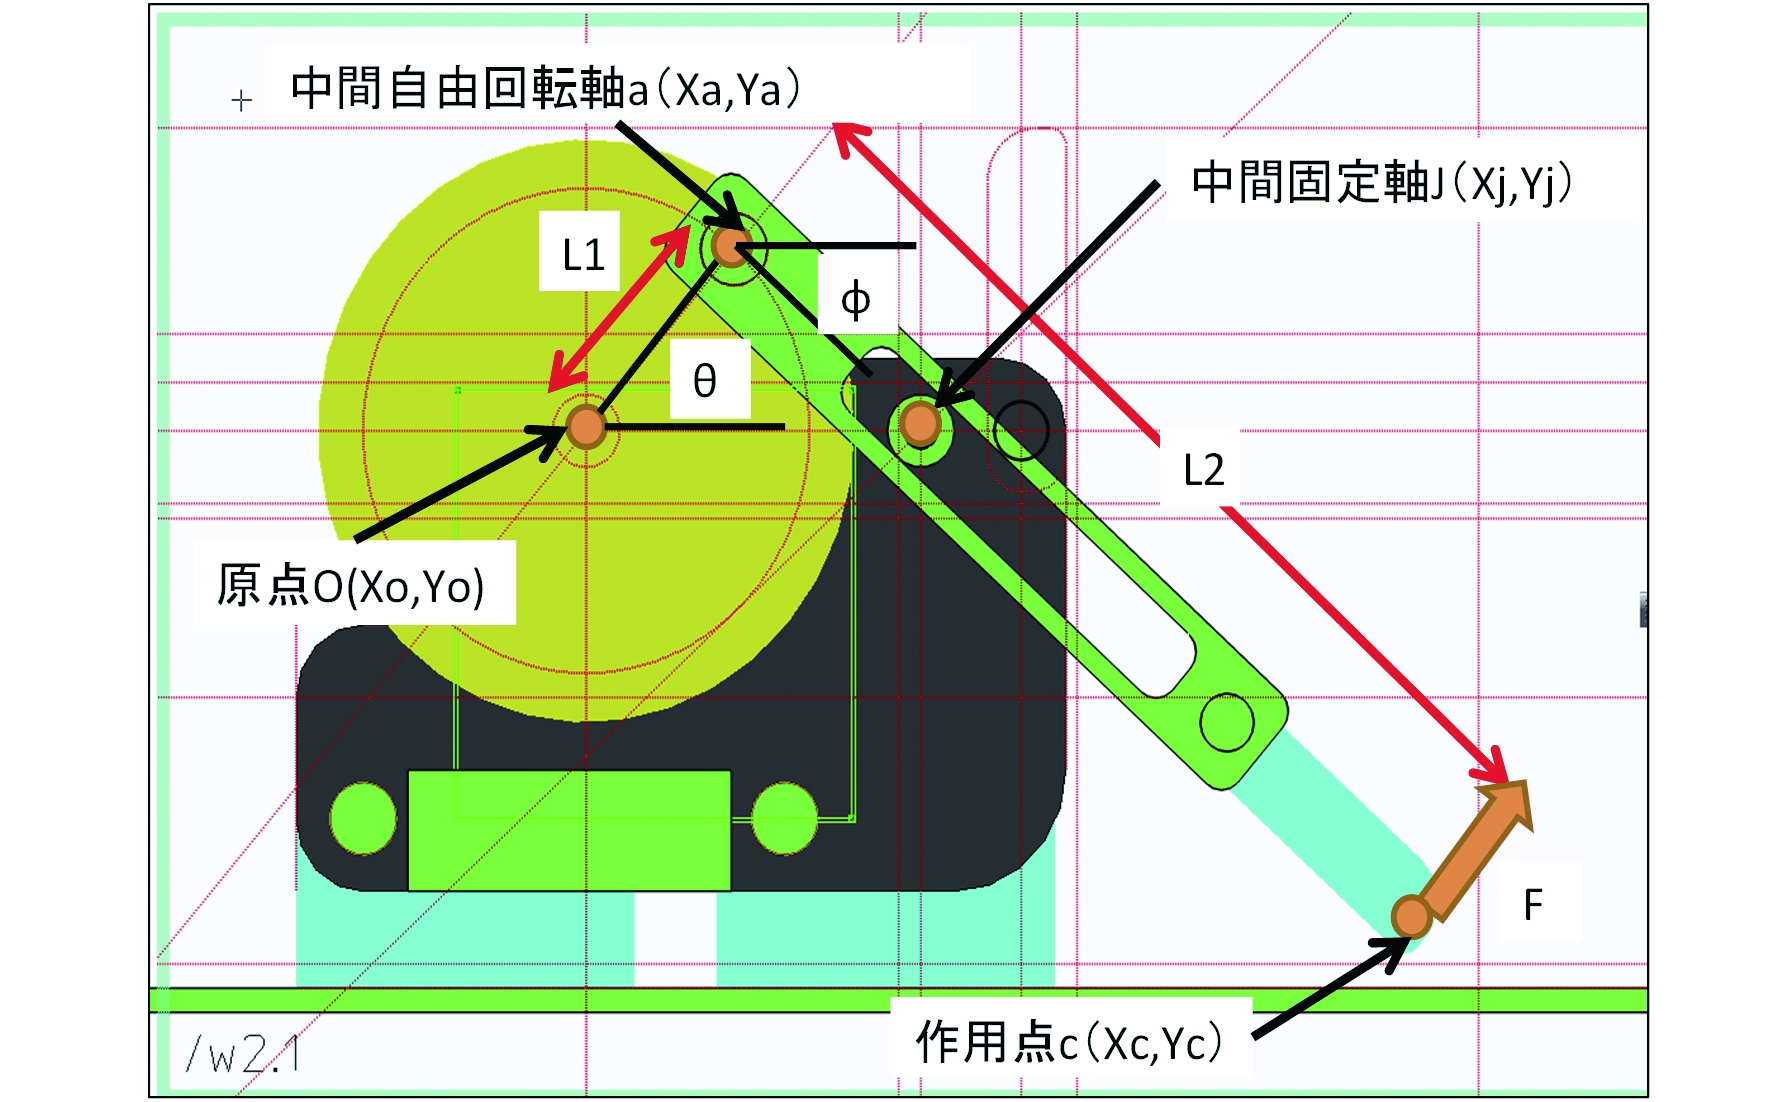
\includegraphics[width=270pt]{fig/fig05_cmyk.jpg}
\caption{アーム 計算モデル}
\label{fig05}
\end{figure}

\clearpage

\subsubsection{アーム設計パラメータ 計算結果とパラメータ決定}\label{ux30a2ux30fcux30e0ux8a2dux8a08ux30d1ux30e9ux30e1ux30fcux30bfux8a08ux7b97ux7d50ux679cux3068ux30d1ux30e9ux30e1ux30fcux30bfux6c7aux5b9a}

\begin{itemize}
\tightlist
\item
  アームの射程距離:作用点位置は機体前面から250mm
\item
  相手機体持ち上げ高さ:大会規格の200mm地点を通過
\item
  相手機体持ち上げ力:作用点で4208gfの力が出る(3500gf以上)
\end{itemize}

\begin{figure}[htbp]
\centering
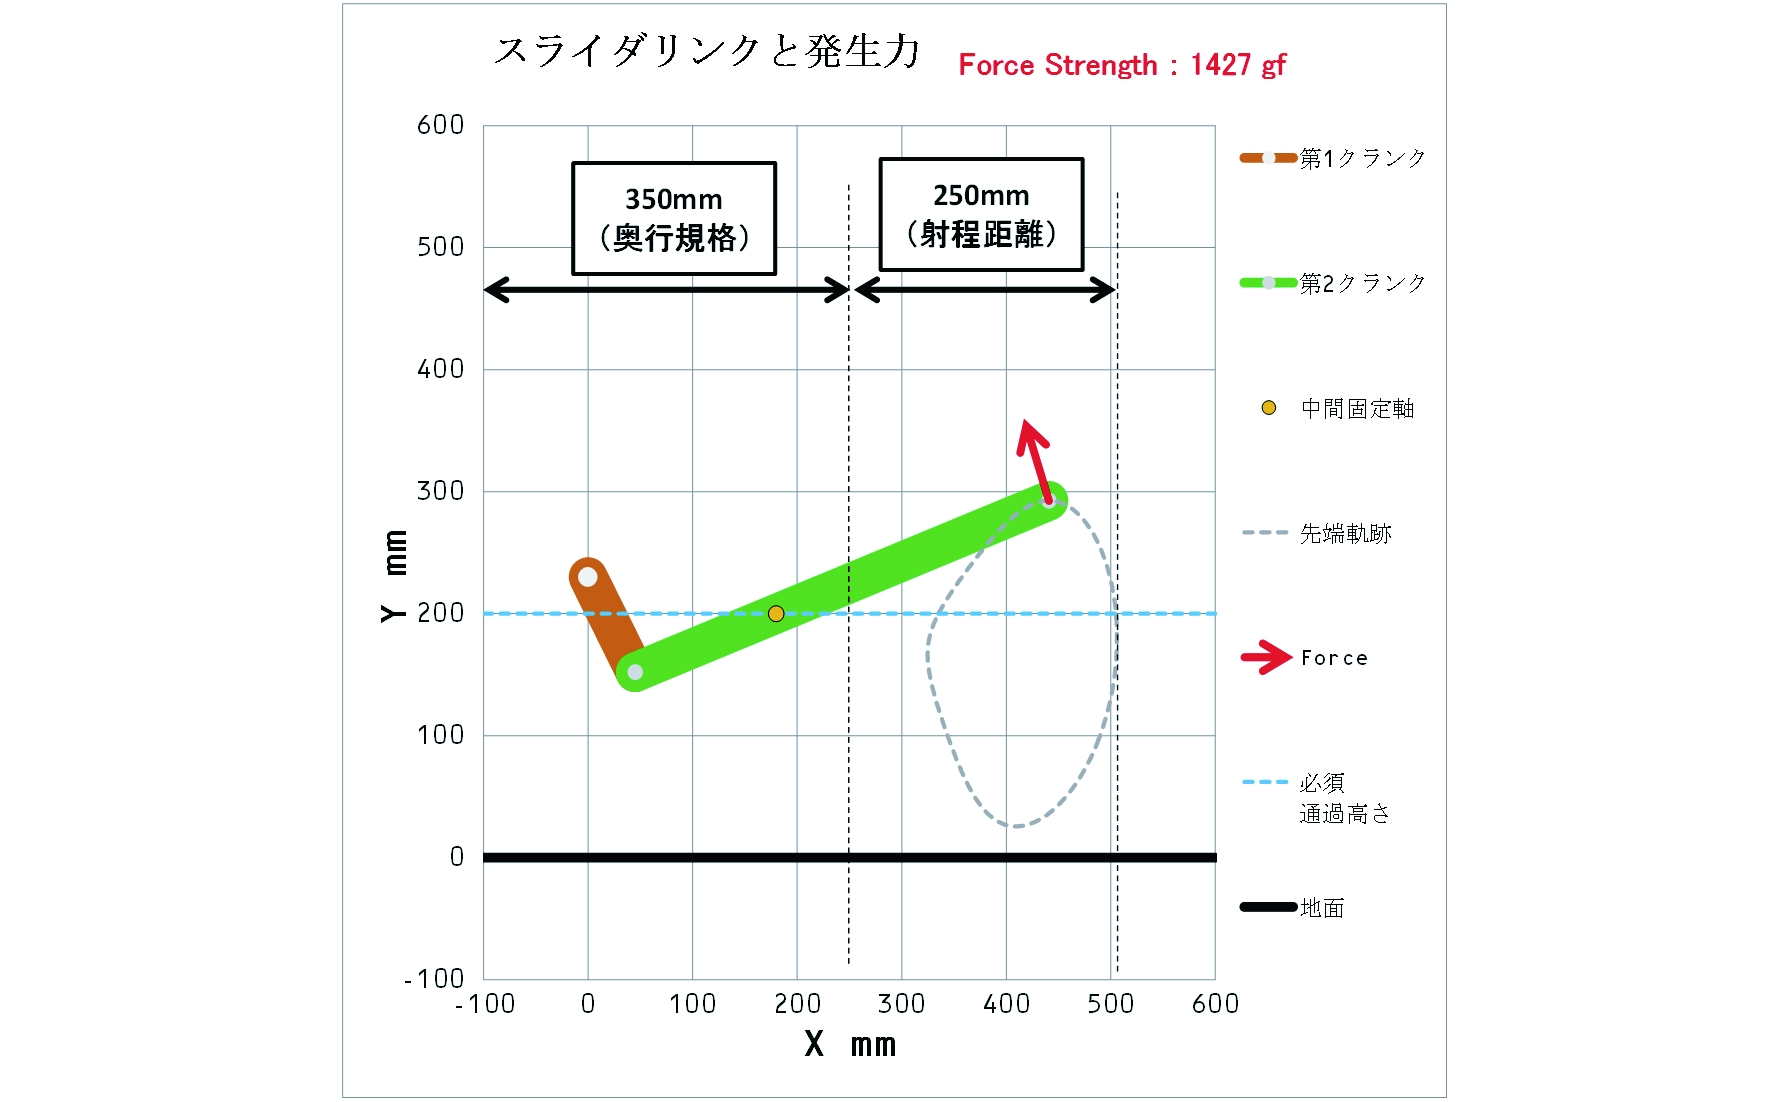
\includegraphics[width=390pt]{fig/fig07_cmyk.jpg}
\caption{アーム 計算結果}
\label{fig07}
\end{figure}

\begin{figure}[htbp]
\centering
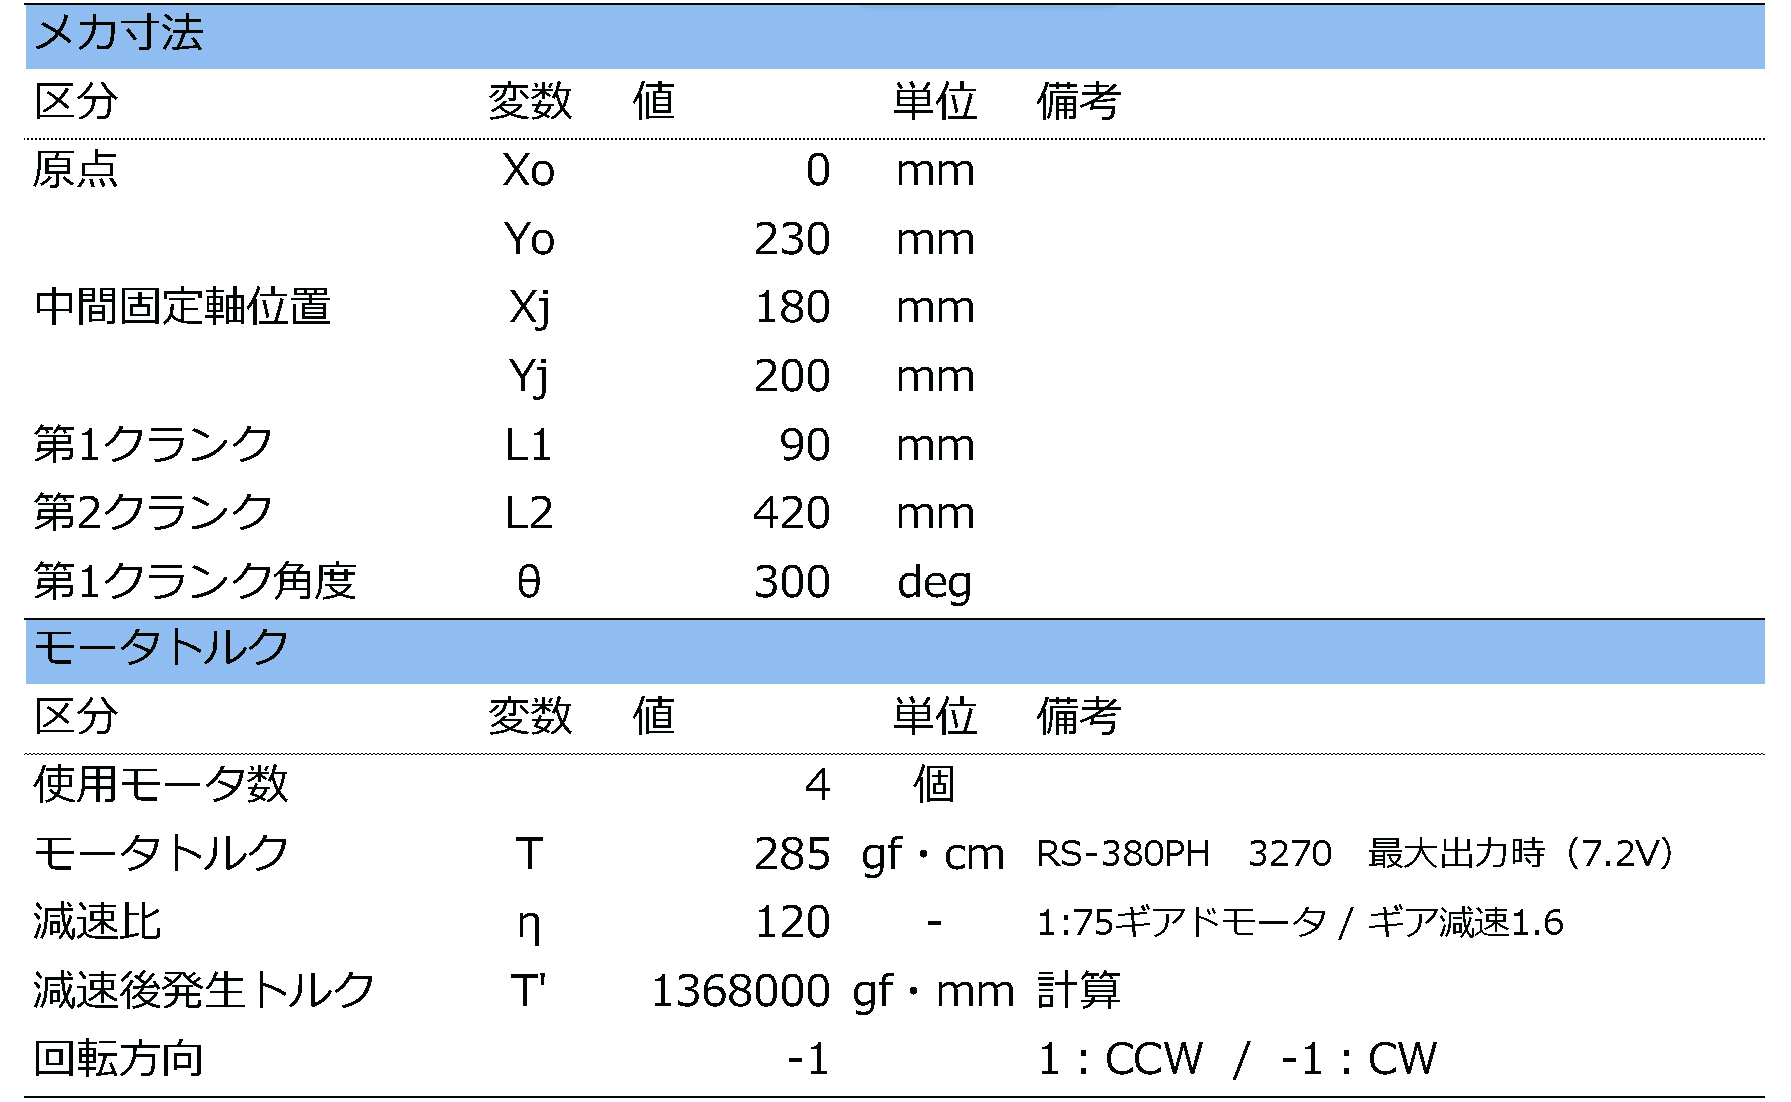
\includegraphics[width=250pt]{fig/fig06_cmyk.jpg}
\caption{アーム 設計パラメータの決定}
\label{fig06}
\end{figure}

\clearpage

\subsection{アーム強度計算}\label{ux30a2ux30fcux30e0ux5f37ux5ea6ux8a08ux7b97}

かわさきロボット競技大会では相手機体とぶつかるアーム部に最も強い力が加わるため、下記のような目標設定をしました

\begin{itemize}
\tightlist
\item
  作用点に3500g(機体重量の大会規格)が加わったときに破壊しないこと
\end{itemize}

計算モデルをFig.\ref{fig08}に示します。
部品名称はFig.\ref{fig05}と同様です。

\begin{itemize}
\tightlist
\item
  中間自由回転軸aを固定端と設定
\item
  作用点に3500gfが加わるように設定
\item
  アームの作用点に力が加わったときの第2クランク部品が中間固定軸から受ける力を計算
\item
  片持ち梁モデル計算からアームに加わる曲げ応力を計算
\item
  安全率は1.5、
  材料強度はABSの30\%と想定(3Dプリンタ樹脂充填率)して許容応力を計算
\end{itemize}

\begin{figure}[htbp]
\centering
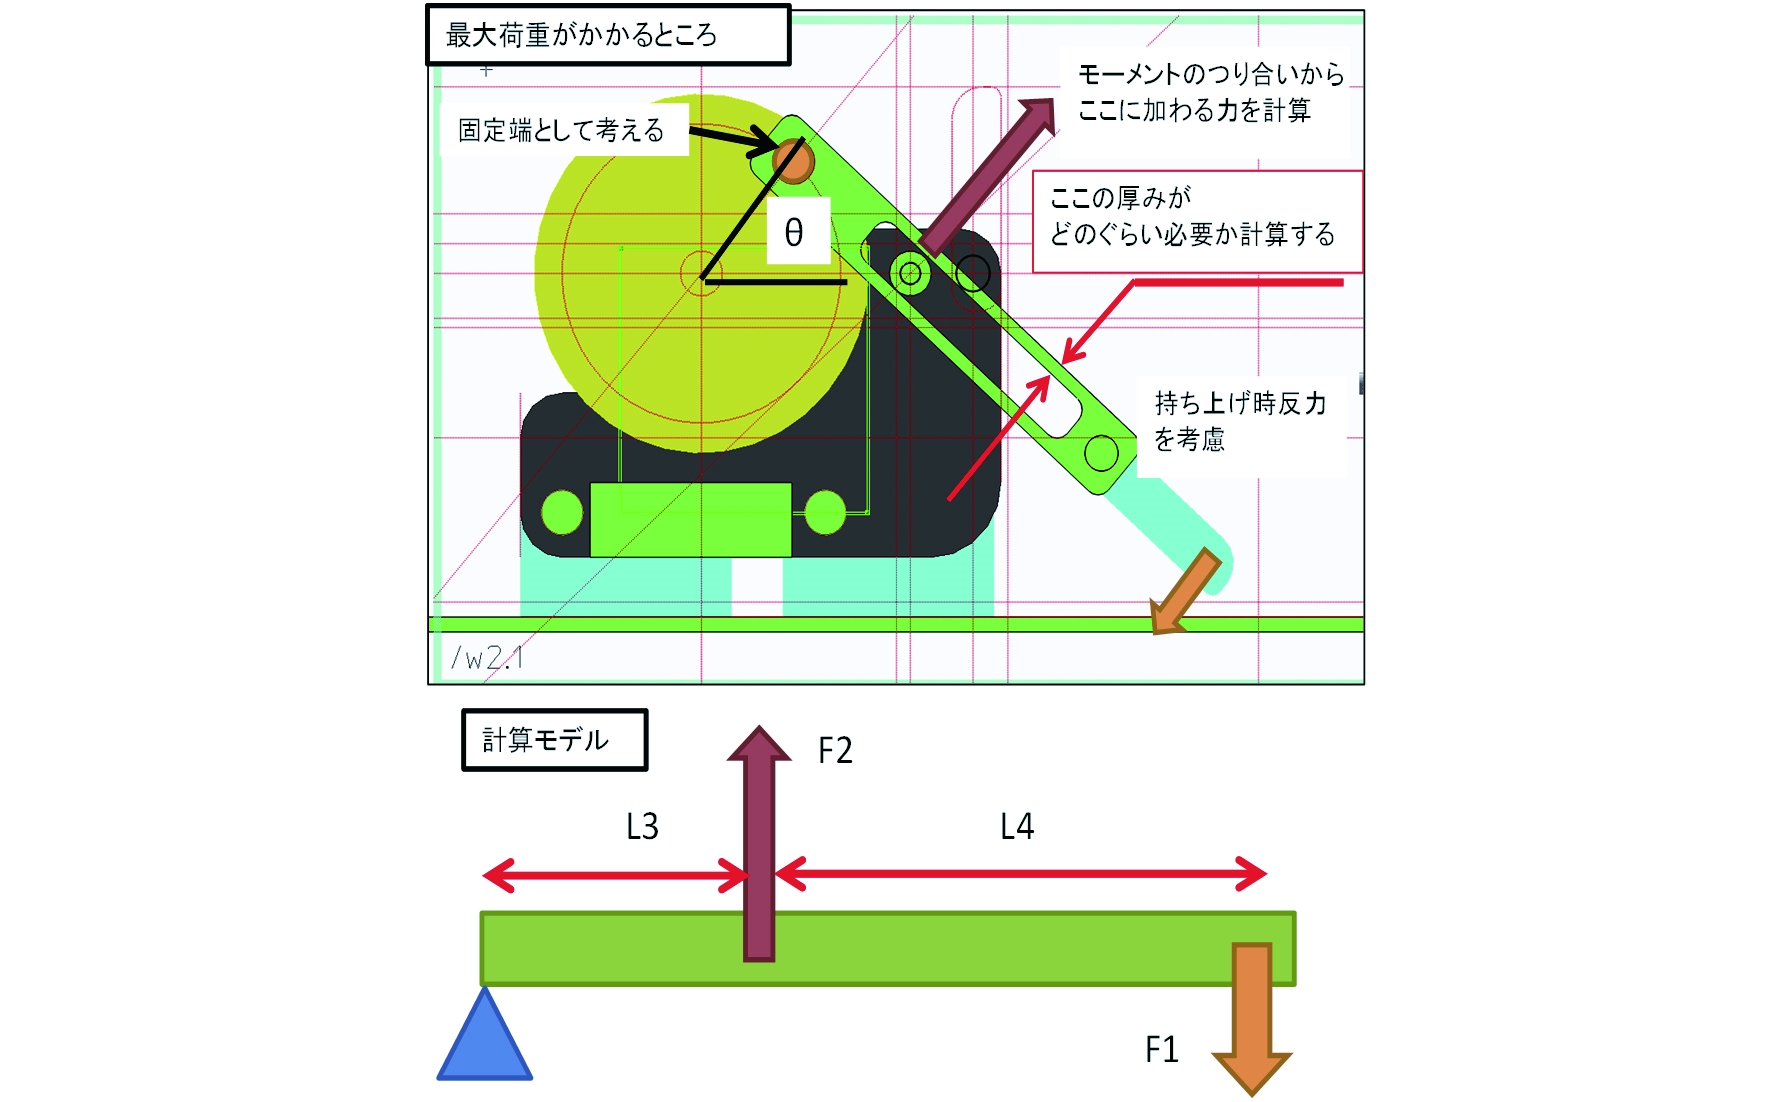
\includegraphics[width=450pt]{fig/fig08_cmyk.jpg}
\caption{強度計算 モデル}
\label{fig08}
\end{figure}

\clearpage

\subsubsection{計算結果とパラメータ設定}\label{ux8a08ux7b97ux7d50ux679cux3068ux30d1ux30e9ux30e1ux30fcux30bfux8a2dux5b9a}

\begin{itemize}
\tightlist
\item
  アームに加わる曲げ応力最大値:500gf/mm\textsuperscript{2}
  (許容曲げ応力:515gf/mm\textsuperscript{2} 以下)
\end{itemize}

\begin{figure}[htbp]
\centering
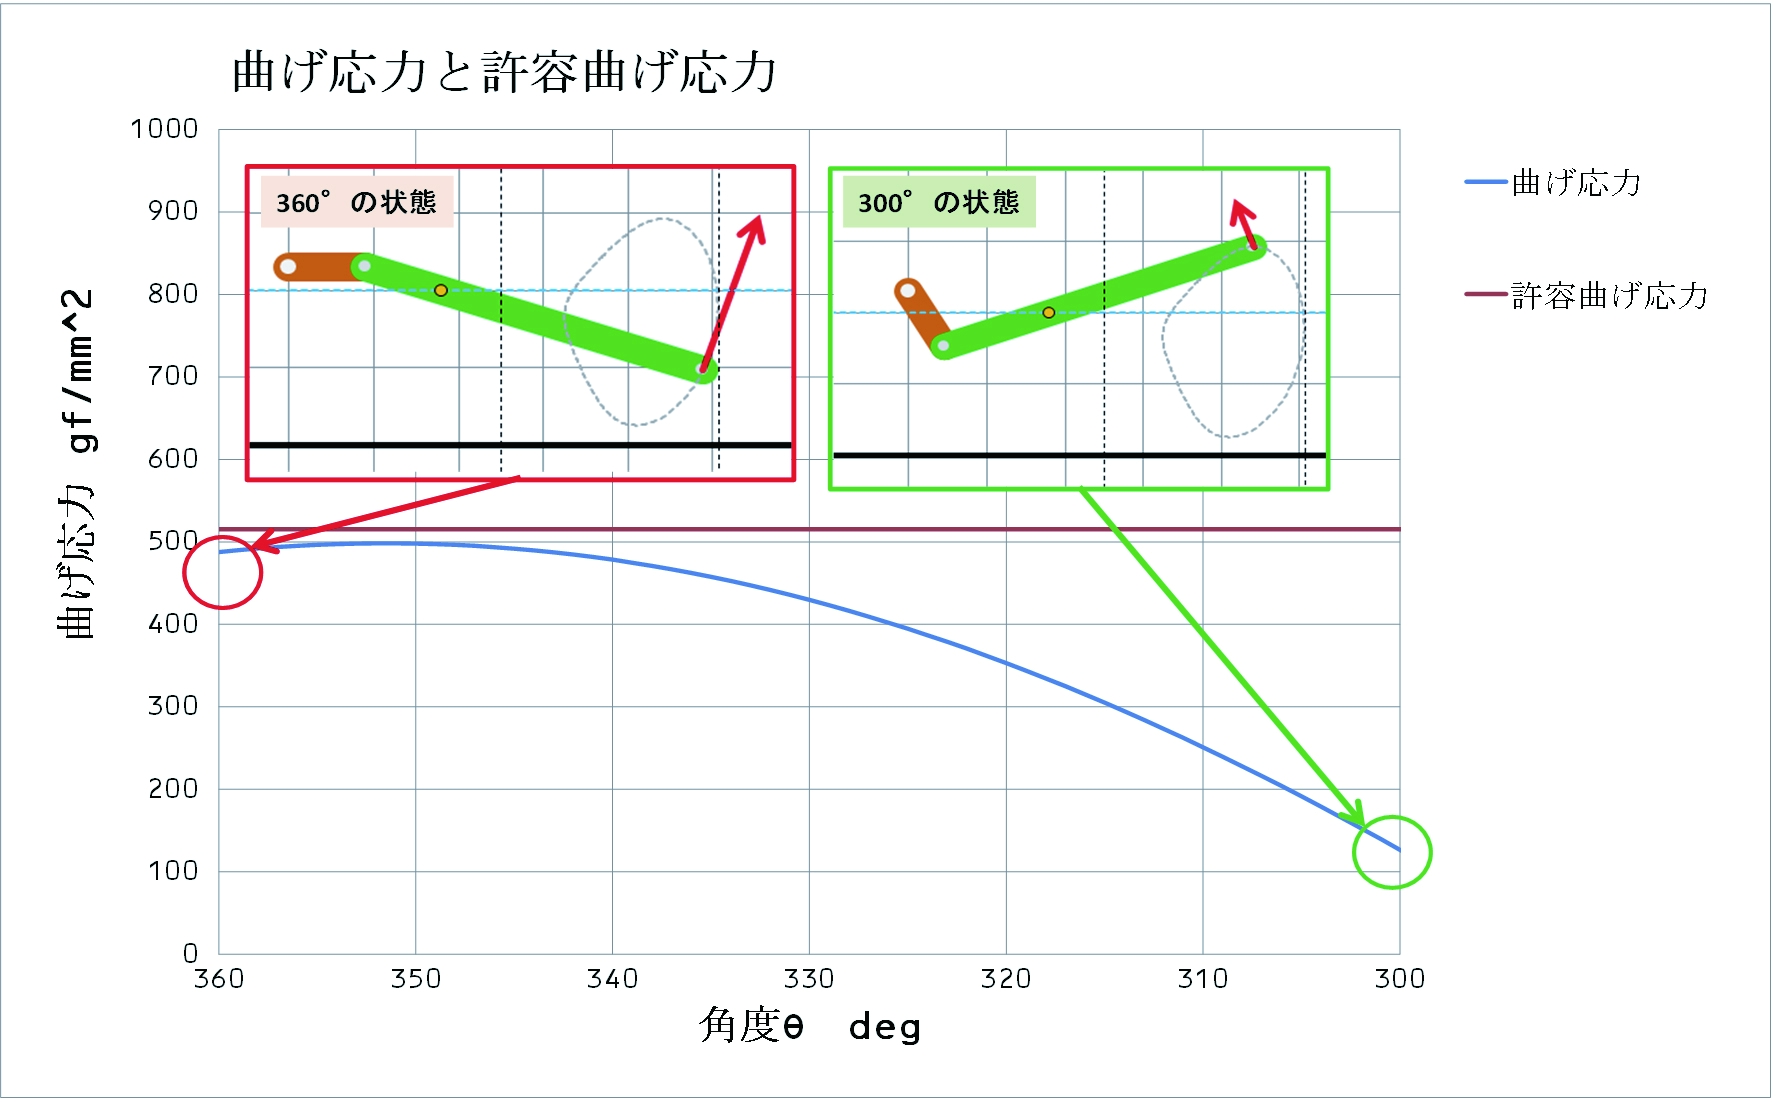
\includegraphics[width=380pt]{fig/fig09_cmyk.jpg}
\caption{強度計算 結果}
\label{fig09}
\end{figure}

上記結果となったときの設計パラメータはFig.\ref{fig10}の通りです。
部品幅を32mm以上、厚みを23mm以上とすればよい、という結果となりました。

\begin{figure}[htbp]
\centering
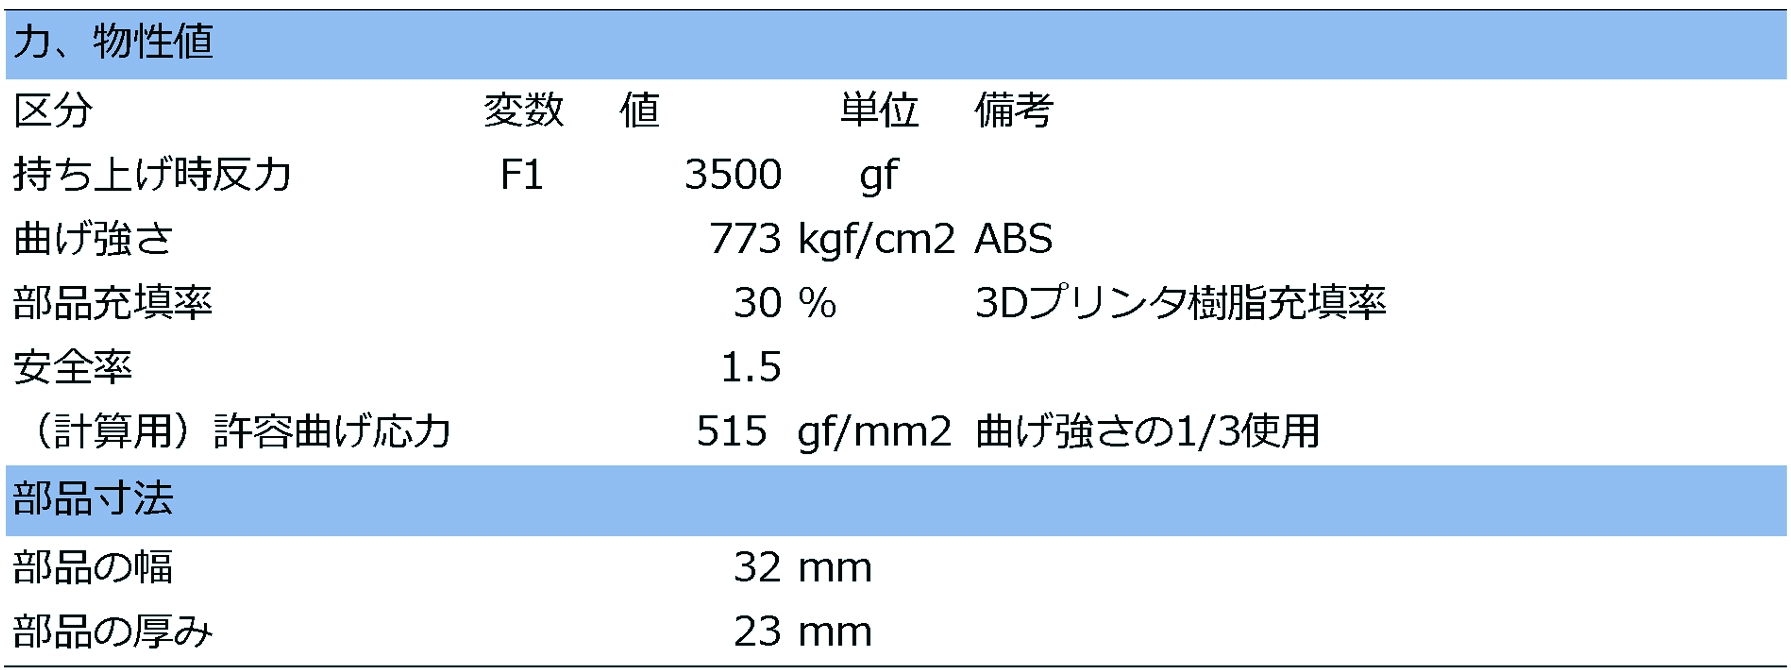
\includegraphics[width=350pt]{fig/fig10_cmyk.jpg}
\caption{強度設計 パラメータ}
\label{fig10}
\end{figure}

\clearpage

\subsection{積層方向の割れ防止構成}\label{ux7a4dux5c64ux65b9ux5411ux306eux5272ux308cux9632ux6b62ux69cbux6210}

第2章のおさらいになりますが、Fig.\ref{fig12}にFDM形式3Dプリンタの部品作成の様子を示します。
一層ずつ積層して形状を作り上げていくため、積層面が剥がれる方向の力に弱いです。

\begin{figure}[htbp]
\centering
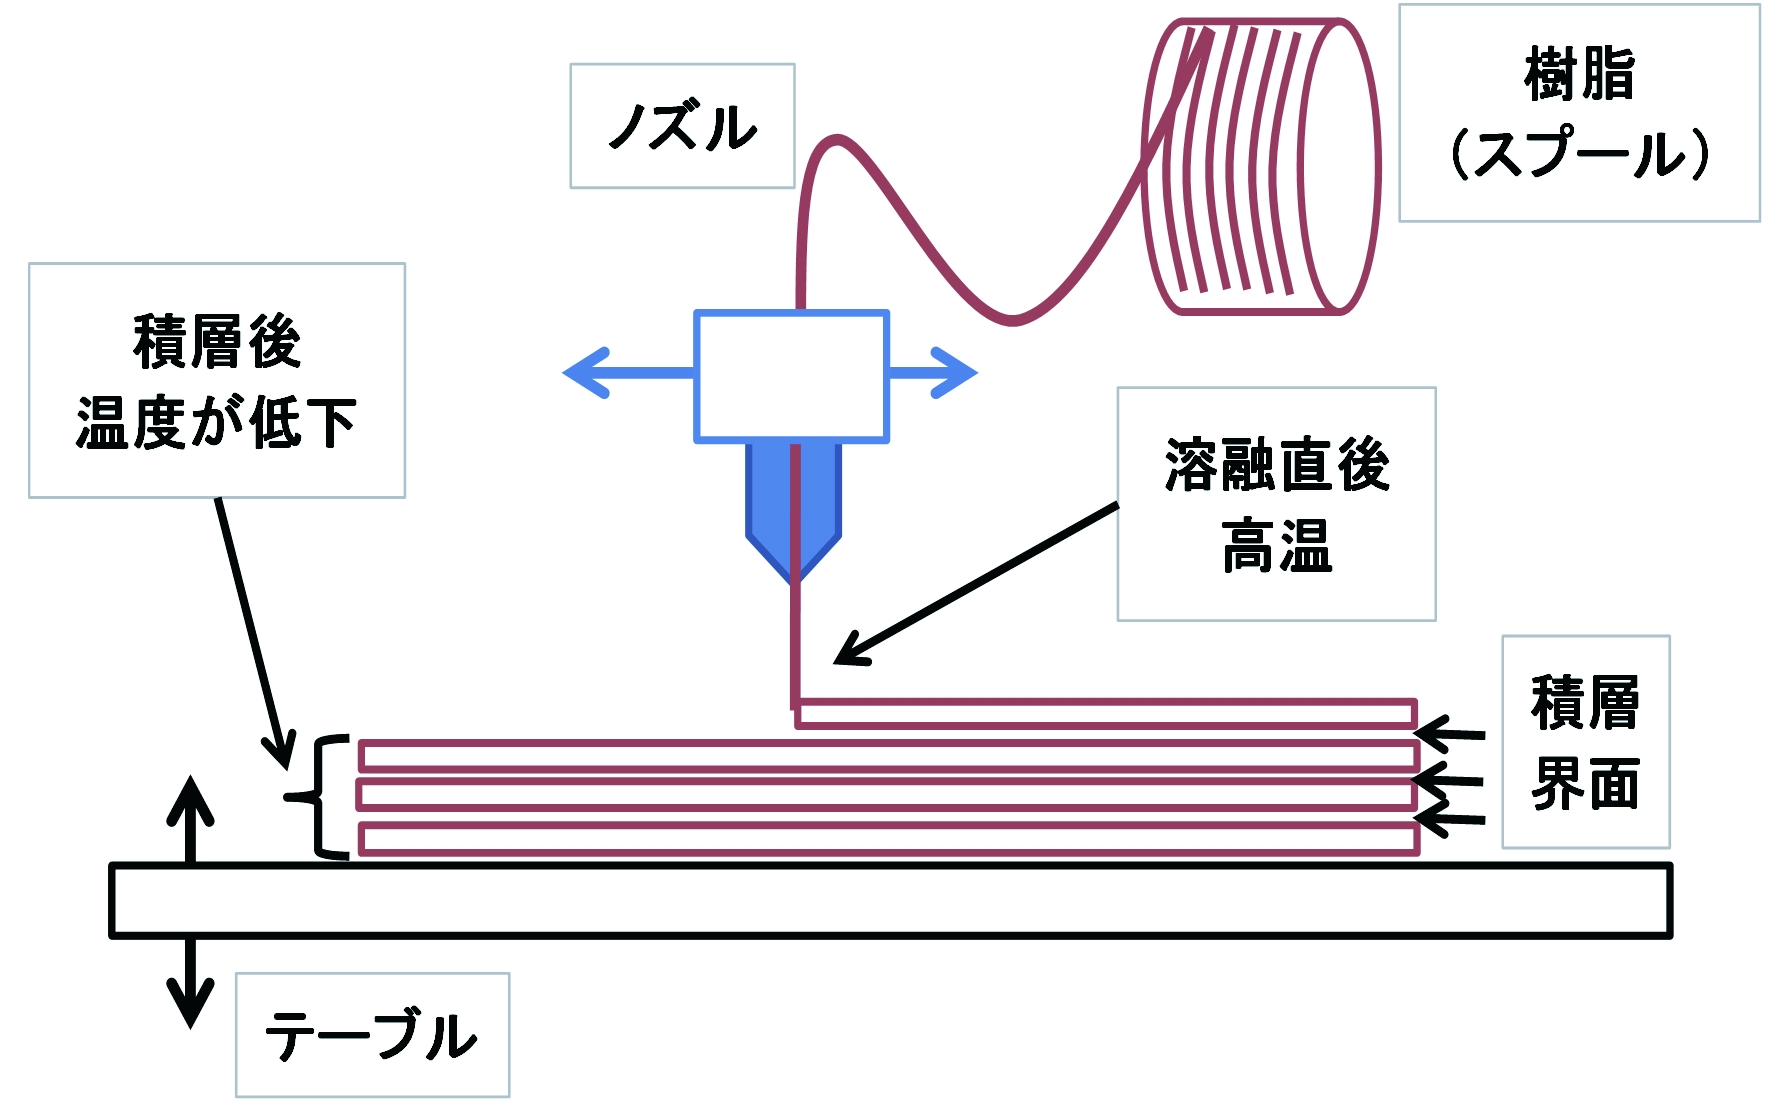
\includegraphics[width=250pt]{fig/fig12_cmyk.jpg}
\caption{3Dプリンタ(FDM方式) 部品作成の様子}
\label{fig12}
\end{figure}

\subsubsection{対策案}\label{ux5bfeux7b56ux6848}

上記のような積層方向に対する剥がれに対する強度は、樹脂温度や積層ピッチ等、様々な影響を受けるため机上計算は困難です。
 
そこで、積層方向に対して大きな力が加わる部品に関しては、できる限り破壊のリスクを減らすため図\ref{fig13}に示す構成を取ることとしました。
まず積層方向に対して力が加わる側の部品Aを中空形状とします。
次に積層方向を90°変更した補強部品Bを別途作成し、部品Aの中空部に圧入します。
この構成を取ることにより、積層方向に対して力が加わったとしても部品Bが力を受けてくれるため破壊しにくくなります。

\begin{figure}[htbp]
\centering
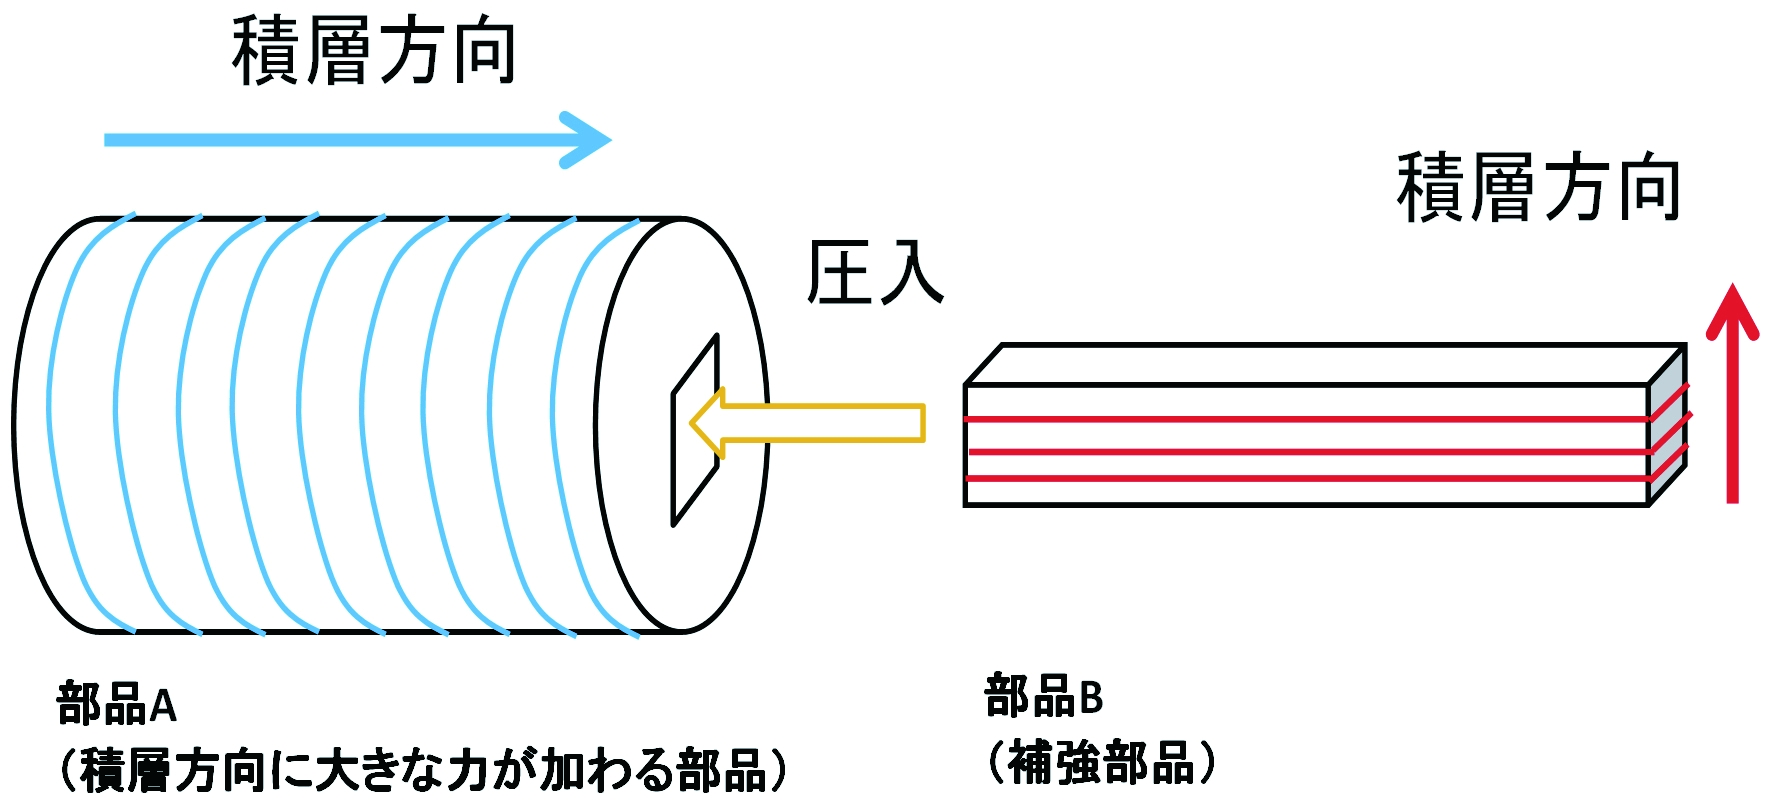
\includegraphics[width=250pt]{fig/fig13_cmyk.jpg}
\caption{積層方向 強度アップ構成}
\label{fig13}
\end{figure}

\clearpage

\subsection{モータ出力部の削れ防止構成}\label{ux30e2ux30fcux30bfux51faux529bux90e8ux306eux524aux308cux9632ux6b62ux69cbux6210}

駆動構成のシンプル化のため、本機体の脚部・アーム部の駆動モータにタミヤのギアドモータ380K\cite{tamiya_380k}を採用することにしました。
ギアドモータの出力部はDカットされた出力軸から駆動を伝達する必要があります。
ギアドモータの出力軸径はφ6mmと細いため、直接3Dプリンタで作成した部品へ駆動を伝達するとFig.\ref{fig14}のようにDカット部で削れが生じます。
削れが進行すると、最悪駆動伝達ができなくなる恐れがあります。

\begin{figure}[htbp]
\centering
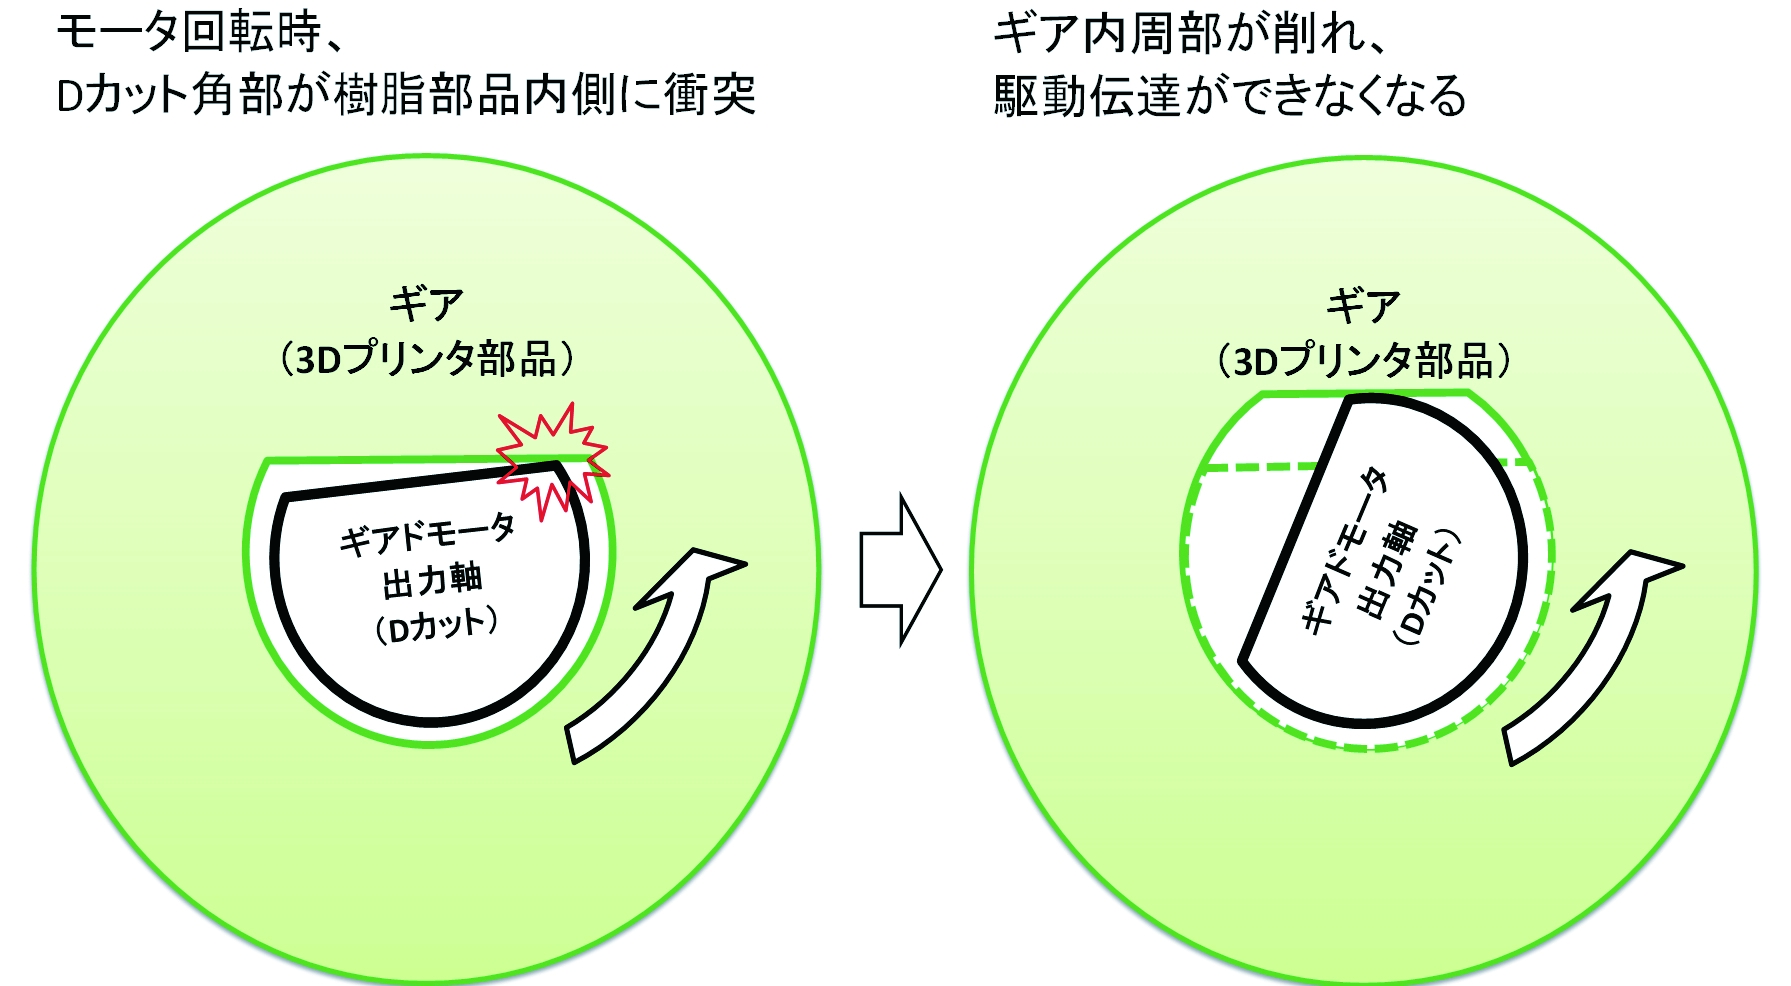
\includegraphics[width=280pt]{fig/fig14_cmyk.jpg}
\caption{ギア削れの様子}
\label{fig14}
\end{figure}

そこで、モータ出力を受け取る部分だけは、金属(今回はアルミ)で部品を作成することとしました。
この金属部品から3Dプリンタで作成した部品へ駆動を伝達することで、モータ出力部の削れを防止します。

\subsection{大型部品の作成方法}\label{ux5927ux578bux90e8ux54c1ux306eux4f5cux6210ux65b9ux6cd5}

3Dプリンタはテーブルサイズ以上のサイズの部品は作ることができません。
私の所有している3Dプリンター\cite{replicator2x}のテーブルサイズは246mm×152mm×155mmです。

一方、かわさきロボット競技大会のサイズ規格は幅250mm×奥行350mm×高さ700mmですので、
テーブルサイズ以上の部品を作るための構成を考えました。

\begin{itemize}
\tightlist
\item
  複数部品を嵌め合わせて大型部品を構成
\item
  強度確保のため厚みを十分に確保
\item
  はめ込み形状を利用して部品同士を結合させる
\item
  ねじれにも強いはめ込み形状
\end{itemize}

実施例詳細は、詳細設計で説明します。
